\chapter{Expériences et résultats}
\label{chap:experiences}

\section{Introduction}
Ce chapitre rassemble les résultats enregistrés pendant le développement. Les cas ratés sont présentés avec les cas réussis, car ils expliquent les changements apportés au modèle et les limites de la solution finale.

\section{Questions et organisation des essais}
Les expériences répondent à trois questions. Le premier modèle peut-il reproduire les commandes du professeur tout en réalisant une formation sans contact ? Le changement de structure du modèle permet-il d'utiliser une commande brute avec plusieurs effectifs ? Enfin, la chaîne hybride de navigation peut-elle déplacer une formation autour d'obstacles proches de ses cibles ?

Les campagnes sont présentées dans leur ordre de développement, car leurs échecs expliquent les choix suivants. Elles n'utilisent pas toutes les mêmes données ni les mêmes conditions. Une amélioration entre deux campagnes ne suffit donc pas à attribuer un gain à un seul composant. À l'intérieur d'une campagne, les contrôleurs comparés partent des mêmes états et utilisent les mêmes critères de réussite.

Les valeurs proviennent des rapports conservés dans le dépôt. Les figures montrent des trajectoires enregistrées et des courbes issues des journaux d'entraînement. Leurs légendes précisent la campagne, le contrôleur et le cas représenté.

\begin{table}[htbp]
\centering\small
\begin{tabularx}{\textwidth}{p{2.5cm}p{3.5cm}X}
\toprule
Campagne & Question principale & Ensemble évalué\\\midrule
Référence multi-formes & Effet du filtre classique & 9 formes réservées, 12 robots\\
Correction & Effet d'exemples sur les états du réseau & 18 cas frais, 12 robots\\
Pilote multi-effectifs & Passage à 24 et 64 robots & 3 formes par effectif\\
Modèle structuré v2 & Mouvement appris sans filtre & 18 cas réservés, 12/24/64 robots\\
Navigation finale & Transport près des obstacles & 8 cas par contrôleur, carré à 12 robots\\
\bottomrule
\end{tabularx}
\caption{Principales campagnes discutées. « Cas » désigne une combinaison de forme, de départ et d'effectif ou de scène ; il ne signifie pas toujours un départ distinct.}
\end{table}

\section{Premier modèle : une imitation correcte ne suffit pas}
Le GAT de référence est entraîné avec douze robots à partir des commandes du professeur. Après sélection des poids sur la validation, neuf formes sont évaluées dans une partition réservée. Les résultats sont présentés dans le Tableau~\ref{tab:reference}. La même configuration initiale est utilisée pour ces formes ; les neuf épisodes ne représentent donc pas neuf tirages de départ indépendants.

\begin{table}[htbp]
\centering\small
\begin{tabular}{lrrrr}
\toprule
Contrôleur & Réussites & Contacts & Erreur finale (m) & Temps (s)\\\midrule
Professeur classique & 9/9 & 0 & 0.00000 & 29.83 \\
GAT de référence brut & 0/9 & 54 & 0.01269 & -- \\
GAT de référence protégé & 9/9 & 0 & 0.01269 & 30.43 \\
\bottomrule\end{tabular}

\caption{Campagne réservée du modèle de référence. Les erreurs et temps sont des moyennes ; le temps porte sur les épisodes réussis. Le tiret indique qu'aucun épisode n'a réussi. Source : rapport 008d.}
\label{tab:reference}
\end{table}

Le professeur réussit les neuf cas sans contact. Le réseau protégé réussit également les neuf, avec une erreur finale moyenne d'environ 1,27 cm. Son temps moyen de stabilisation est de 30,43 s, contre 29,83 s pour le professeur. Ces temps comprennent la préparation et l'attribution.

Le réseau brut atteint presque la même erreur finale moyenne, mais provoque 54 événements de contact et ne réussit aucun cas. Cet écart est le résultat principal de la campagne : observer uniquement la dernière image aurait conduit à une conclusion trompeuse. Les robots peuvent finir près des places demandées après s'être touchés pendant le mouvement. Le filtre classique a donc une contribution importante à la réussite du système protégé.

La MSE de validation, égale à 0,112516 pour les poids retenus, mesure l'imitation de commandes sur des exemples. Elle ne remplace pas cette évaluation du déplacement. Les états rencontrés par le réseau peuvent aussi s'éloigner progressivement de ceux du professeur, même si les premières erreurs de commande sont modestes.

\section{Collecte de correction : moins de contacts, mais toujours des échecs}
Une collecte complémentaire interroge le professeur sur des états rencontrés par le modèle. Le nouvel entraînement donne davantage de poids aux situations proches d'un voisin. L'évaluation suivante utilise neuf formes et deux graines fraîches, soit 18 cas.

Sur ces mêmes cas, le modèle brut initial provoque 102 contacts. Le modèle corrigé en provoque 65, soit une baisse d'environ 36,3\,\%. Les deux restent à zéro réussite sur dix-huit. La version corrigée avec protection réussit les dix-huit cas sans contact.

La correction a donc un effet mesurable, mais elle n'atteint pas l'objectif d'un mouvement brut sans contact. Nous ne la présentons pas comme un modèle sûr. Les poids corrigés et les trajectoires ratées sont conservés pour expliquer cette conclusion, tandis que le modèle de référence protégé reste disponible pour la démonstration hybride.

\section{Premier essai avec plusieurs effectifs}
Le pilote multi-effectifs utilise 12, 24 et 64 robots. Les dimensions de l'espace, de la forme et de la préparation sont adaptées à chaque profil. Trois formes sont réservées au test pour chaque effectif. Les résultats sont :

\begin{table}[htbp]
\centering
\begin{tabular}{rrrrr}
\toprule
Robots & Brut : réussites & Brut : contacts & Protégé : réussites & Protégé : contacts\\\midrule
12 & 2/3 & 1 & 3/3 & 0\\
24 & 0/3 & 65 & 0/3 & 0\\
64 & 0/3 & 127 & 0/3 & 0\\\bottomrule
\end{tabular}
\caption{Pilote multi-effectifs avant le modèle structuré. Source : rapport 012.}
\label{tab:pilote}
\end{table}

À 24 et 64 robots, le système protégé évite les contacts dans ces cas mais ne termine pas correctement le protocole. Le rassemblement ne permet pas d'aboutir à l'attribution attendue. Une absence de collision n'est donc pas suffisante pour déclarer une réussite.

Ce pilote montre aussi qu'un réseau qui accepte un nombre variable de voisins n'est pas automatiquement performant avec un effectif plus grand. Les interactions, les dimensions et la durée des phases changent. La bonne valeur de la perte de validation du pilote ne résout pas ces difficultés en exécution.

\section{Modèle structuré : formation à 12, 24 et 64 robots}
\subsection{Validation avant le test réservé}
La première version structurée réussit six des neuf cas de validation, avec six contacts dans les trois cas restants. Ces échecs ne sont pas écartés du bilan. L'entraînement de la seconde version renforce la pénalité de séparation et utilise une marge plus grande. Cette seconde version réussit ensuite les neuf cas de validation, portant sur le triangle, la lettre B et le nombre 7 aux trois effectifs.

Les poids sont alors fixés avant l'exécution du test réservé. Ce test utilise le rectangle, la lettre C et le nombre 3, avec les graines 8500 et 8501 à chacun des effectifs 12, 24 et 64. Cela donne dix-huit cas, mais seulement six configurations de départ distinctes : deux par effectif, réutilisées pour trois formes. La conclusion statistique doit rester proportionnée à cette diversité.

\subsection{Résultats du test réservé}
Le Tableau~\ref{tab:vector} rassemble les résultats du GAT structuré brut. Dans les dix-huit cas, aucun contact n'est observé et aucun filtre de sécurité n'intervient pendant les phases de mouvement apprises. Le professeur, évalué sur les mêmes départs, réussit lui aussi les dix-huit cas sans contact.

\begin{table}[htbp]
\centering\small
\begin{tabular}{rrrrrr}
\toprule
Robots & Réussites & Contacts & Erreur finale (m) & Temps GAT (s) & Temps réf. (s)\\\midrule
12 & 6/6 & 0 & $1.79\times10^{-7}$ & 29.43 & 30.00 \\
24 & 6/6 & 0 & $3.44\times10^{-7}$ & 85.23 & 85.23 \\
64 & 6/6 & 0 & $8.67\times10^{-7}$ & 465.80 & 465.93 \\
\bottomrule\end{tabular}

\caption{Test réservé du GAT structuré v2. Les erreurs et temps sont des moyennes sur six cas par effectif. Les temps incluent toutes les phases de préparation. Source : rapport 014.}
\label{tab:vector}
\end{table}

Les erreurs finales sont très faibles, de l'ordre de $10^{-7}$ à $10^{-6}$ m. Elles sont obtenues après une longue stabilisation dans une simulation sans bruit. Elles ne doivent pas être lues comme une précision atteignable par des robots physiques. Pour la mission, le critère utile reste le respect du seuil de 0,1 m, du seuil de vitesse, du maintien et de l'absence de contact.

L'audit des 36 trajectoires, dix-huit pour chaque contrôleur, vérifie les mises à jour physiques, les bornes, les contacts, l'attribution, la fenêtre de stabilisation et l'identité des départs comparés. Il vérifie aussi que les fichiers utilisent les poids retenus. La plus petite distance entre centres observée pendant le déplacement interpolé est d'environ 0,546 m à douze robots, 0,516 m à vingt-quatre et 0,411 m à soixante-quatre. La distance de 0,5 m choisie pendant l'apprentissage n'est donc pas toujours maintenue. L'absence de contact dans ces cas ne constitue pas une garantie générale sur cette marge.

\begin{figure}[htbp]
\centering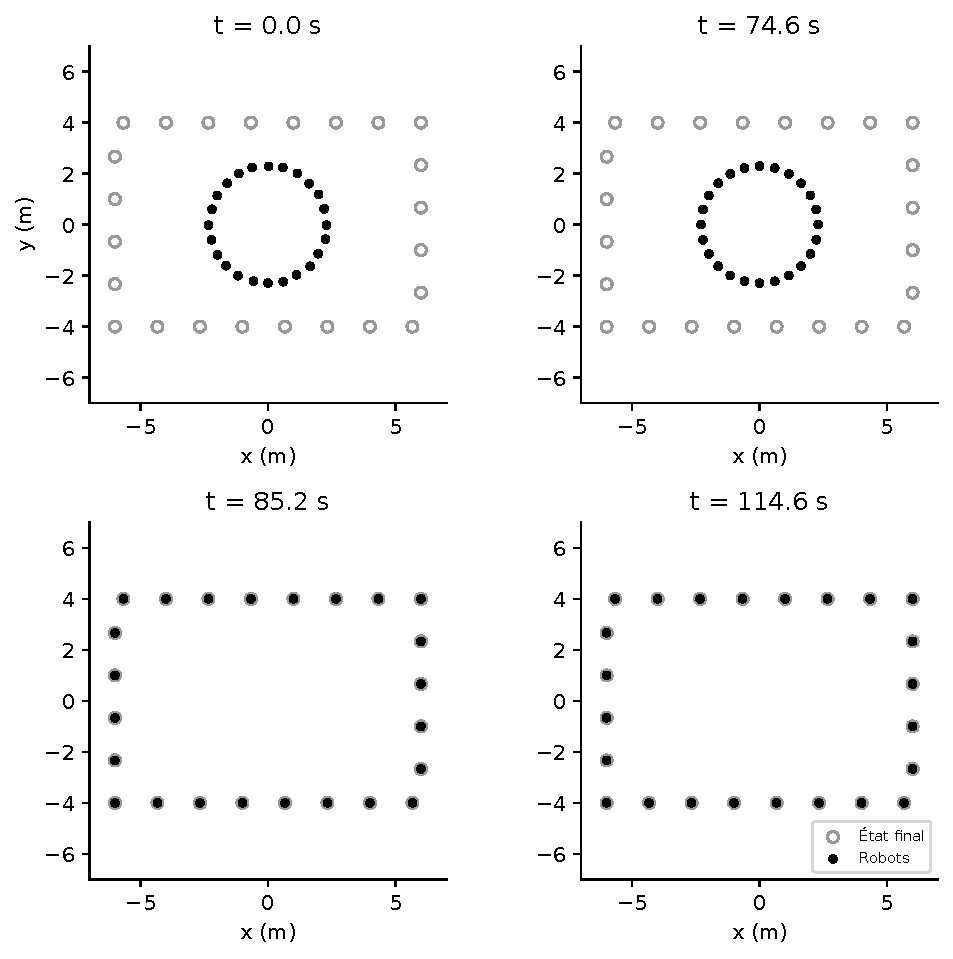
\includegraphics[width=\textwidth]{images/current_sequence.pdf}
\caption{Quatre états d'une trajectoire enregistrée du rectangle à 24 robots, graine 8500, GAT structuré brut. Les cercles vides indiquent les positions finales enregistrées, les points pleins les robots à l'instant indiqué. Le cercle initial est une étape du protocole.}
\label{fig:sequence}
\end{figure}

\subsection{Pourquoi le temps augmente-t-il autant ?}
Le temps moyen atteint 465,8 s à 64 robots. Il s'agit du temps simulé depuis le début de la mission, et non du temps de calcul d'une décision du réseau. Le budget d'attribution vaut à lui seul 409,6 s à cet effectif. Les phases de rassemblement et de freinage ajoutent 32 s, et le mouvement vers la forme commence à 441,6 s. À 24 robots, il commence à 74,6 s ; à 12 robots, à 24,4 s.

\begin{figure}[htbp]
\centering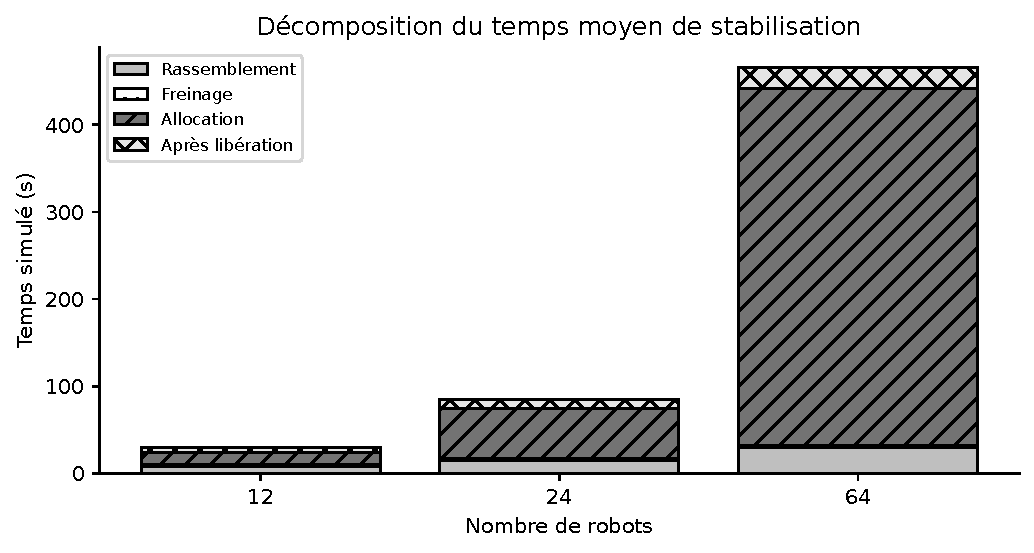
\includegraphics[width=.88\textwidth]{images/current_timing.pdf}
\caption{Temps de stabilisation décomposé à partir du protocole et des moyennes mesurées du GAT structuré. L'allocation domine à 64 robots. La dernière partie couvre le temps entre la libération du mouvement et la stabilisation.}
\label{fig:temps}
\end{figure}

Cette lecture change l'interprétation du résultat. Le réseau ne met pas plus de quatre cents secondes à calculer une accélération. Le protocole attend de nombreux tours d'échanges avant de lancer le mouvement final. Réduire ce budget demanderait un travail sur l'attribution et sa condition d'arrêt, puis une nouvelle vérification des trajectoires.

\section{Transitions entre formes}
Une mission peut demander plusieurs formes successives. Le système conserve alors les positions et les vitesses entre les étapes. Il ne replace pas les robots directement sur la forme suivante. Les annonces d'attribution sont renouvelées pour la nouvelle mission, et l'enregistrement permet de vérifier cette continuité.

Les campagnes de transitions du GAT de référence protégé et du professeur comprennent un pilote de six séquences puis une validation de deux séquences par contrôleur. Les séquences validées réussissent sans contact. Les huit étapes présentes dans les deux séquences de validation ne sont pas huit expériences indépendantes : l'état de chaque étape dépend de la précédente. Ces résultats concernent les contrôleurs évalués dans cette campagne, et non une validation supplémentaire du GAT structuré brut.

\section{Navigation et obstacles proches des cibles}
\subsection{Difficulté et correction du trajet}
Les premières expériences de navigation ont rencontré des cas sans stabilisation malgré l'absence de contact. Le déplacement du seul centre ne tenait pas suffisamment compte de la largeur de la formation. Un autre cas demandait de placer un robot sur une cible occupée par un obstacle. Ces deux situations appelaient des réponses différentes : préparer un détour pour la première, refuser la destination impossible pour la seconde.

Le planificateur corrigé vérifie le déplacement de toutes les places autour des obstacles. Une campagne ultérieure sur trois formes et des parcours complémentaires réussit huit cas par contrôleur, sans contact. Une dernière campagne rapproche ensuite les obstacles des cibles et conserve les mêmes exigences de réussite. Les résultats de cette dernière campagne sont détaillés ci-dessous ; ils ne remplacent pas rétroactivement les échecs des scènes antérieures.

\subsection{Campagne finale}
Les essais finaux portent sur un carré de largeur 6 m à douze robots. Le centre de référence se déplace de $(-1,0)$ à $(1,0)$ m. Les scènes à plusieurs obstacles contiennent de cinq à dix disques. Les centres des obstacles sont situés à au plus un mètre d'une place finale du carré. Leur disposition est définie dans le programme ; il ne s'agit pas de cartes tirées au hasard dans un environnement inconnu.

La campagne comporte les six nombres d'obstacles, de cinq à dix, avec la graine 8901 ; elle ajoute dix obstacles avec la graine 8902 et un cas à un obstacle avec cette même graine. Cela représente huit cas pour le professeur et huit pour le GAT de référence protégé. Pour les sept cas à plusieurs obstacles, la préparation est classique et commune ; la différence de contrôleur concerne le transport. Le cas à un obstacle vérifie également le comportement de la chaîne déjà disponible.

\begin{table}[htbp]
\centering\small
\setlength{\tabcolsep}{3pt}
\begin{tabular}{lrrrr}
\toprule
Contrôleur & Réussites & Contacts & Déformation max. (m) & Destination max. (m)\\\midrule
Professeur classique & 8/8 & 0 & $3{,}06\times10^{-11}$ & $1{,}11\times10^{-16}$\\
GAT de référence protégé & 8/8 & 0 & 0,010388 & 0,005550\\\bottomrule
\end{tabular}
\caption{Campagne finale avec obstacles proches des cibles. Les deux dernières colonnes sont les maxima entre les cas, et non des moyennes. La déformation est mesurée pendant le transport. Source : rapport 019.}
\label{tab:navigation}
\end{table}

Les huit cas réussissent pour chacun des deux contrôleurs. L'audit de seize trajectoires confirme la physique et les métriques. Le GAT protégé reste à environ 1,04 cm de déformation maximale et 0,56 cm d'erreur maximale de destination. Ces résultats évaluent une chaîne hybride : planification classique sur carte connue, préparation classique dans les scènes multiples, commande locale et filtre. Ils ne démontrent pas que le réseau a appris à contourner dix obstacles.

\begin{figure}[htbp]
\centering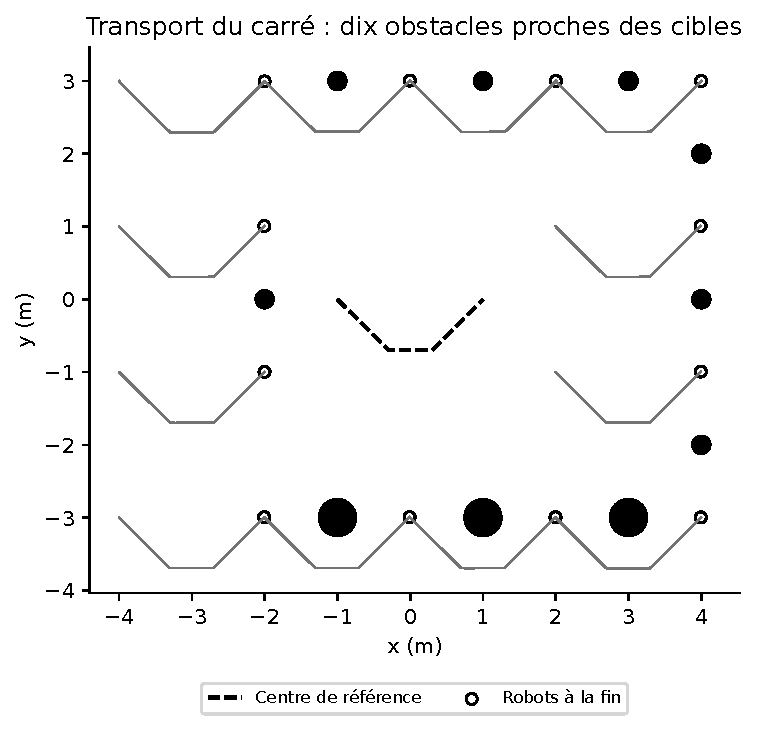
\includegraphics[width=.92\textwidth]{images/current_navigation.pdf}
\caption{Trajectoires enregistrées pendant le transport du carré avec dix obstacles, graine 8901, GAT de référence protégé. Les disques noirs représentent les obstacles à leur rayon physique. Les traits gris suivent les centres des robots ; les cercles vides indiquent leur état final. Le trait discontinu suit le centre de référence. La préparation n'est pas tracée.}
\label{fig:navigation}
\end{figure}

\section{Lecture d'ensemble}
Trois constats ressortent des expériences. D'abord, la qualité de l'imitation mesurée par une MSE n'assure pas la réussite d'une trajectoire : le premier modèle peut finir près de la forme après plusieurs contacts. Ensuite, la structure de la commande et les données de proximité jouent un rôle important dans le développement du modèle brut. La seconde version atteint l'objectif sur les dix-huit cas réservés, mais dans des conditions contrôlées. Enfin, les réussites de navigation dépendent explicitement du planificateur et du filtre classiques.

Les expériences ne suffisent pas à isoler l'effet de l'attention. Plusieurs éléments ont changé entre le premier réseau et le modèle structuré : la représentation, la commande nominale, les données et la fonction de coût. Une comparaison qui retire uniquement les messages, répétée avec plusieurs entraînements et de nouveaux départs, reste nécessaire pour mesurer cet apport séparément.

Les résultats actuels ne valident pas non plus toutes les combinaisons proposées dans l'interface. Les effectifs 8 et 16, certaines formes ou certaines dimensions peuvent être exécutés à titre exploratoire, mais ils ne disposent pas de la même campagne réservée que les profils 12/24/64. De même, un résultat classique à 64 robots ne prouve rien sur un réseau si aucun réseau n'a été utilisé. Le nom du contrôleur et le domaine de validation doivent accompagner chaque démonstration.

\section{Conclusion partielle}
Les essais établissent une réussite du modèle structuré dans son domaine contrôlé et une réussite de la navigation hybride dans les scènes finales. Ils montrent aussi les limites du premier modèle brut et du pilote multi-effectifs. La discussion suivante examine la portée de ces constats.
